\begin{figure}[htbp]
\centering
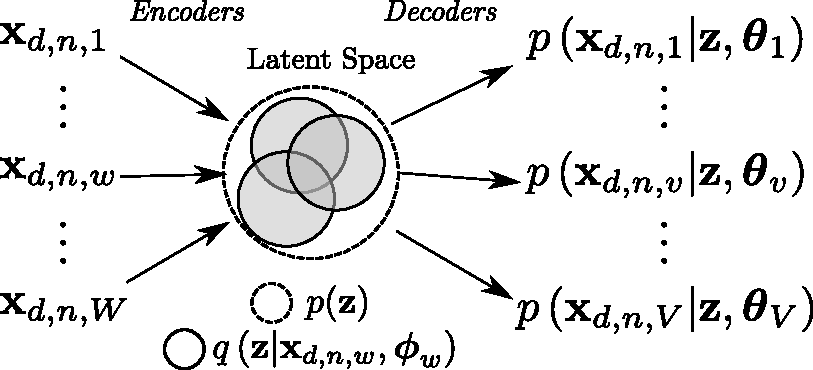
\includegraphics[width=\columnwidth]{./tex/fig/architecture.pdf}
\caption{
General variational framework for our multi-view model.
For every pair of views $v$ and $w$ there is a prediction path $v \leftarrow w$ composed by two learnable functions: the encoding distribution $\q{\z|\xb_w, \phib_w}$ and the decoding likelihood $\p{\xb_v|\z, \thetab_v}$.
Parameters $\phib_w$ and $\thetab_v$ are optimized through \eqnref{eq:argmax} to maximize the likelihood of our generative model under the encoding distributions, and at the same time minimize the Kullback-Leibler distance between every encoder and the prior $\pz$.
To leave the notation uncluttered, in this representation we dropped the dataset index $d$ and data-point $n$ used in the text.
}
\label{fig:architecture}
\end{figure}
